\documentclass[11pt,landscape]{article}
\usepackage[a4paper,top=0cm,left=0cm,right=0cm,bottom=0cm]{geometry}
\usepackage{tikz}
\usepackage{amsmath}
\usepackage{varwidth}
\usepackage{enumitem}
\usepackage[hidelinks]{hyperref}

%%%%%%%%%%%%%%%%%%%%%%%%%%%%%%%%%%%%%%%%%%%%%
% used for cross referencing descriptions
\makeatletter
\def\namelabel#1#2%
    {
      \begingroup%
      #2%
      \def\@currentlabel{#2}%
      \phantomsection\label{#1}
      \endgroup
    }
\makeatother
%%%%%%%%%%%%%%%%%%%%%%%%%%%%%%%%%%%%%%%%%%%%%


\usetikzlibrary{shadows,arrows,positioning,shapes.geometric}
% Define the layers to draw the diagram
\pgfdeclarelayer{background}
\pgfdeclarelayer{foreground}
\pgfsetlayers{background,main,foreground}

%%%%%%%%%%%%%%%%%%%%%%%%%%%%%%%%%%%%%%%%%%%%%%%%%%%%%%%%%%%%%%%%%%%%%%%%%%%%%%%%%%%%%%%%%%
% Define block styles
%%%%%%%%%%%%%%%%%%%%%%%%%%%%%%%%%%%%%%%%%%%%%%%%%%%%%%%%%%%%%%%%%%%%%%%%%%%%%%%%%%%%%%%%%%
\tikzstyle{MODdescript}=[draw, fill=blue!20, text width=20.0em, text centered,
  minimum height=1.5em,drop shadow]
 % \tikzstyle{raute}=[draw, fill=green!20, text width=6.0em,]
\tikzstyle{modules} = [MODdescript, text width=14em, minimum width=10em,
  minimum height=3em, rounded corners, drop shadow]
\tikzstyle{line} = [draw, thick, color=black!50, -latex']
\tikzstyle{interface} = [draw, fill=green!20, node distance=2.5cm, drop shadow]
\tikzstyle{ToImplement}=[draw, fill=red!10, text centered, text width=14em, minimum width=10em,minimum height=3em, rounded corners, drop shadow]
\tikzstyle{ToImplementDescript}=[MODdescript, fill=red!10]

%%%%%%%%%%%%%%%%%%%%%%%%%%%%%%%%%%%%%%%%%%%%%%%%%%%%%%%%%%%%%%%%%%%%%%%%%%%%%%%%%%%%%%%%%%


% Define distances for bordering
\newcommand{\blockdist}{1.3}
\newcommand{\edgedist}{1.5}

\newcommand{\opc}{\alpha}
\newcommand{\epsi}{\psi}
\newcommand{\eb}[1]{\epsi^{(#1)}}
\newcommand{\aM}{\underline{C}}
\newcommand{\msl}{M_\text{sl}} % number of smearing levels

% Draw background
\newcommand{\background}[5]{%
  \begin{pgfonlayer}{background}
    % Left-top corner of the background rectangle
    \path (#1.west |- #2.north)+(-0.5,0.25) node (a1) {};
    % Right-bottom corner of the background rectanle
    \path (#3.east |- #4.south)+(+0.5,-0.25) node (a2) {};
    % Draw the background
    \path[fill=yellow!20,rounded corners, draw=black!50, dashed]
      (a1) rectangle (a2);
      \path (#3.east |- #2.north)+(0,0.25)--(#1.west |- #2.north) node[midway] (#5-n) {};
      \path (#3.east |- #2.south)+(0,-0.35)--(#1.west |- #2.south) node[midway] (#5-s) {};
      \path (#3.east |- #2.north)+(0.7,0)--(#3.east |- #4.south) node[midway] (#5-w) {};
  \end{pgfonlayer}}


\begin{document}
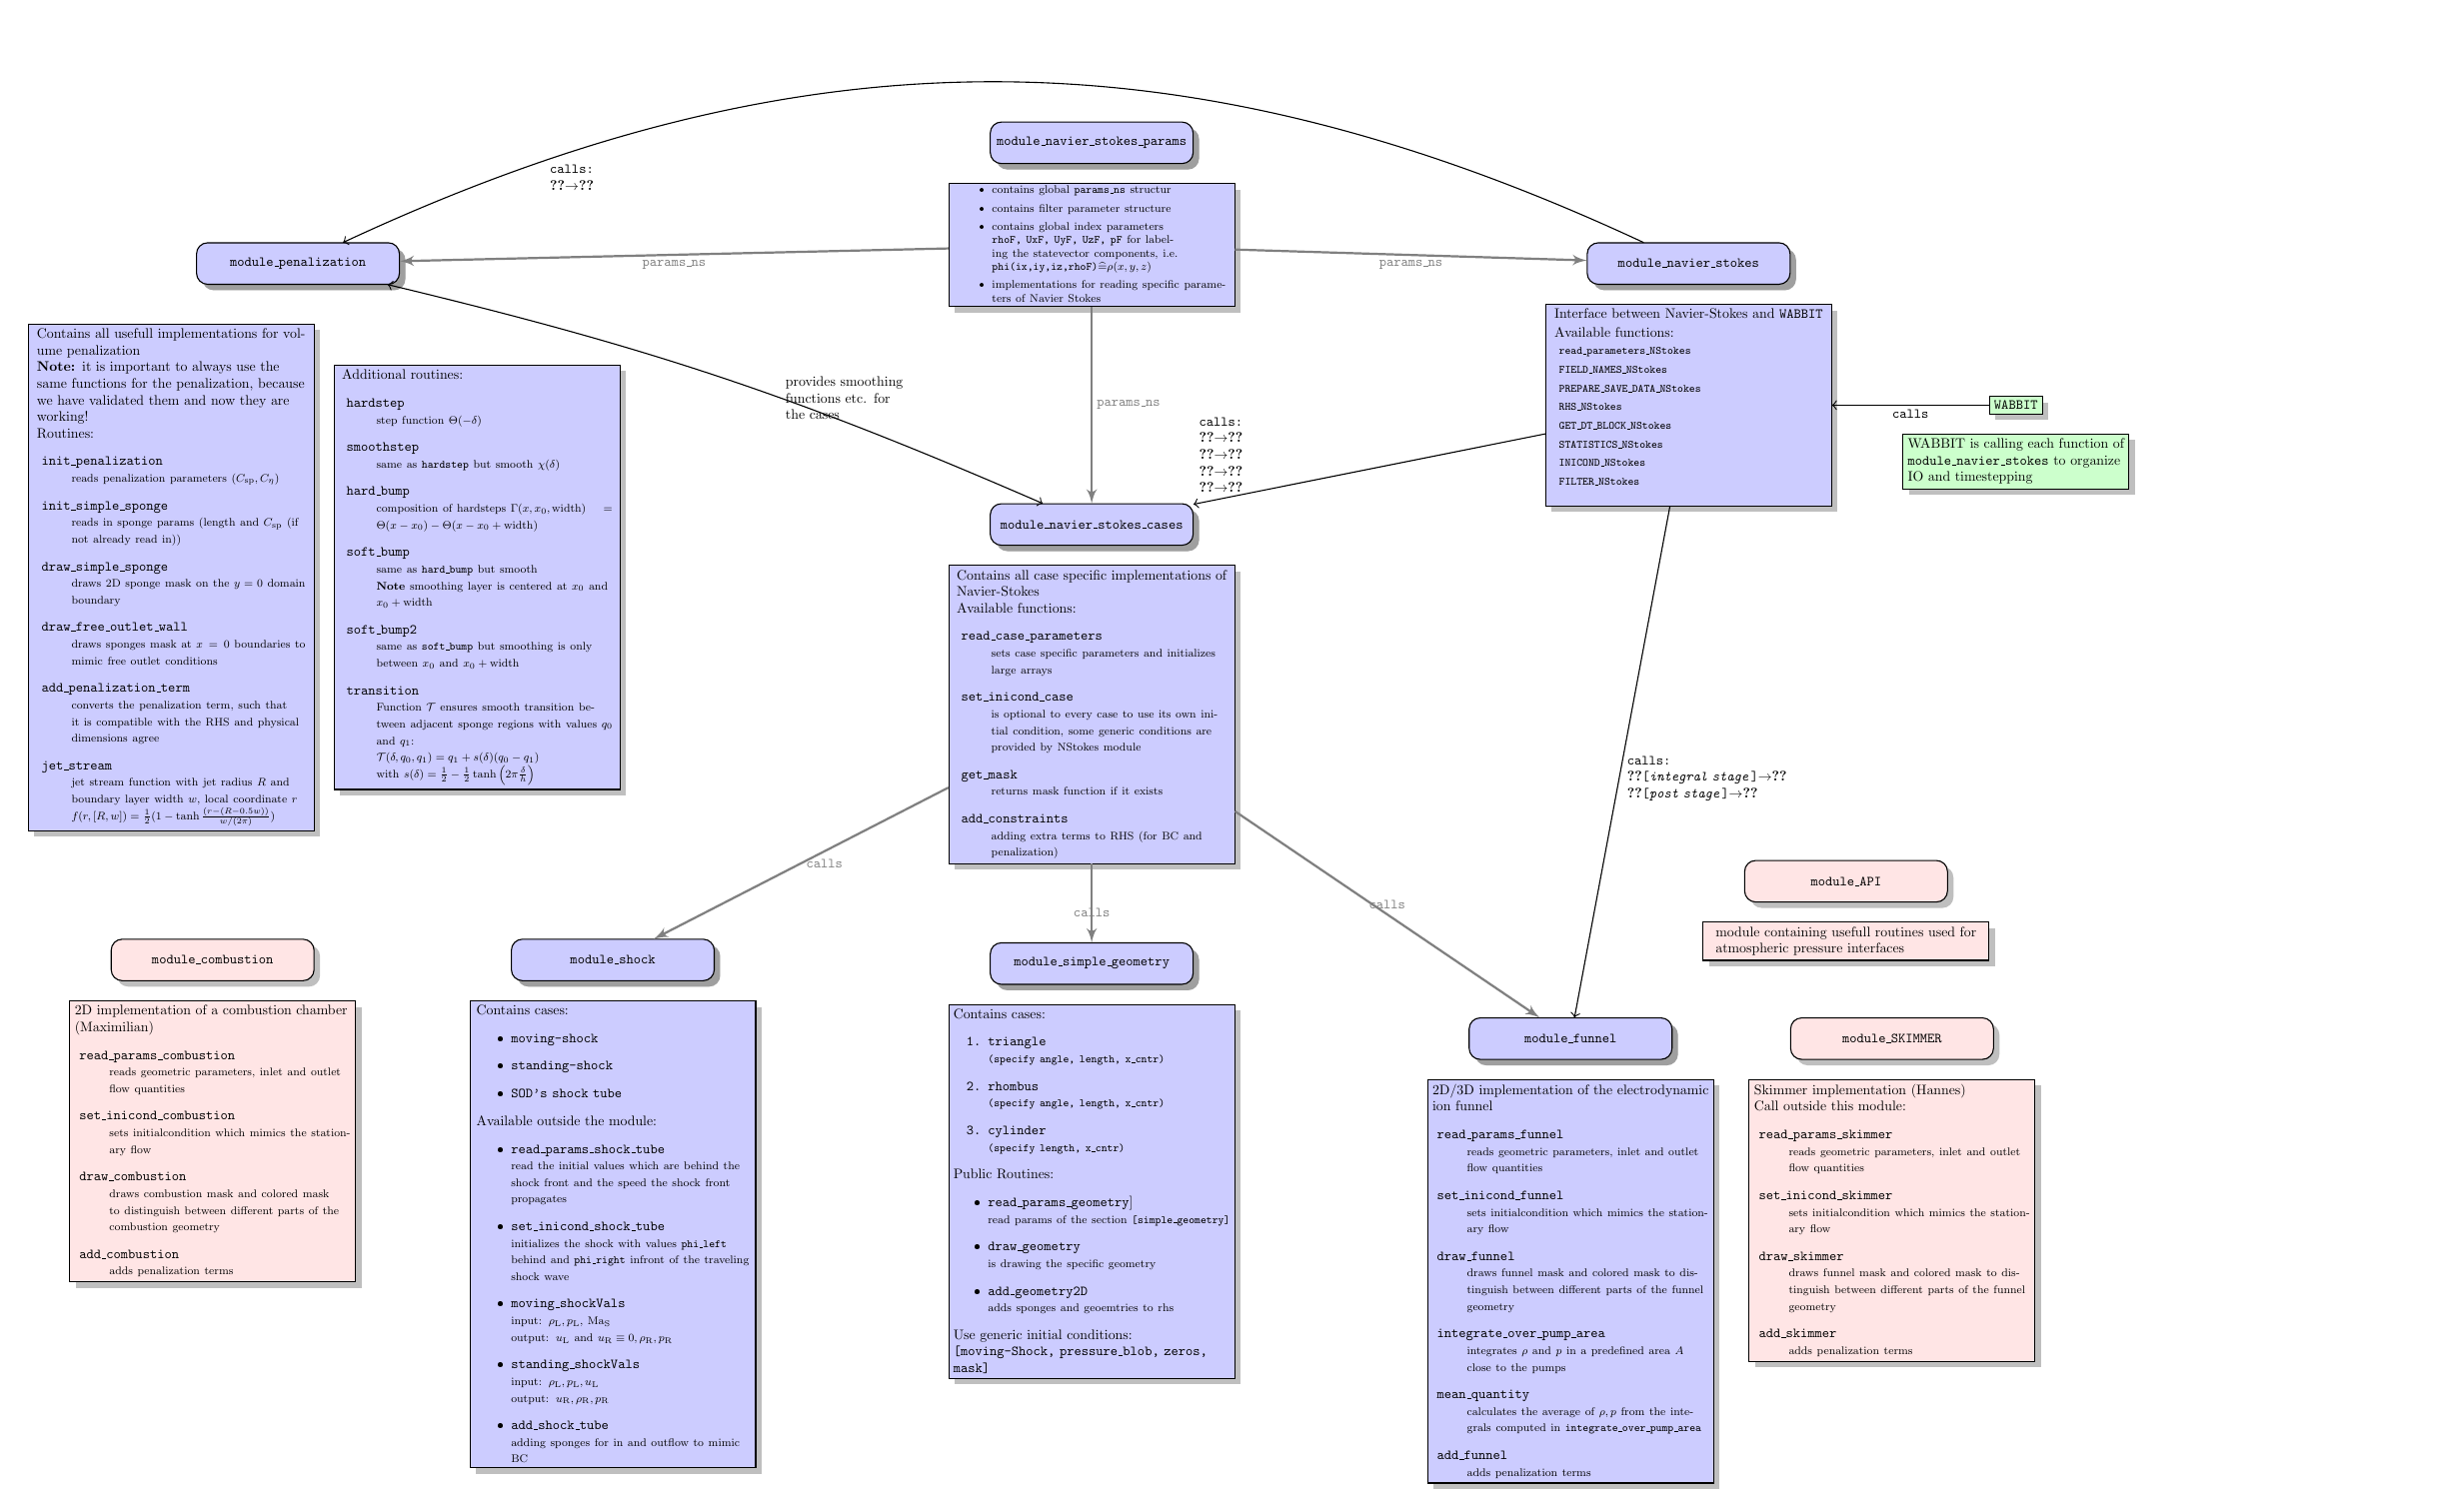
\begin{tikzpicture}[scale=0.5,transform shape,node distance=2.5cm]

  \node (NSPARAMS)  [modules] {\texttt{module\_navier\_stokes\_params}};
  \node (NS-PARAMS-TEXT) [MODdescript,below=0.5cm of NSPARAMS]
{
  \begin{varwidth}{\linewidth} \footnotesize
    \begin{itemize}
        \item  contains global \texttt{params\_ns} structur
        \item  contains filter parameter structure
        \item  contains global index parameters \texttt{rhoF, UxF, UyF, UzF, pF} for labeling
        the statevector components, i.e. \texttt{phi(ix,iy,iz,rhoF)}$\widehat{=}\rho(x,y,z)$
        \item { implementations for reading specific parameters of Navier Stokes}
        \end{itemize}
  \end{varwidth}
};

%%%%%%%%%%%%%%%%%%%%%%%%%%%%%%%%%%%%%%%%%%%%%%%%%%%%%%%%%%%%%%%%%%%%%%%%%%%%%%%%%%%%%%%%%
% PENALIZATION
%%%%%%%%%%%%%%%%%%%%%%%%%%%%%%%%%%%%%%%%%%%%%%%%%%%%%%%%%%%%%%%%%%%%%%%%%%%%%%%%%%%%%%%%%
\node (PENALIZATION)   [modules,below left=2cm and 15cm of NSPARAMS] {\texttt{module\_penalization}};
\node (PENALIZATION-DESC1) [MODdescript,below left=1cm and -3cm of PENALIZATION]
{
\begin{varwidth}{\linewidth}
  Contains all usefull implementations for volume penalization\\
  \textbf{Note:} it is important to always use the same functions for the penalization,
  because we have validated them and now they are working!\\
  Routines:
  \begin{description}
    \item[\namelabel{itm:PENAL0}{\tt init\_penalization}]$\,$\\
    {\footnotesize reads penalization parameters ($C_\mathrm{sp}, C_\eta$)}
    \item[\namelabel{itm:PENAL1}{\tt init\_simple\_sponge}]$\,$\\
    {\footnotesize reads in sponge params (length and $C_\text{sp}$ (if not already read in))}
    \item[\namelabel{itm:PENAL2}{\tt draw\_simple\_sponge}]$\,$\\
    {\footnotesize draws 2D sponge mask on the $y=0$ domain boundary }
    \item[\namelabel{itm:PENAL3}{\tt draw\_free\_outlet\_wall}]$\,$\\
    {\footnotesize draws sponges mask at $x=0$ boundaries to mimic free outlet conditions}
    \item[\namelabel{itm:PENAL4}{\tt add\_penalization\_term}]$\,$\\
    {\footnotesize converts the penalization term, such that it is compatible with the RHS and physical dimensions agree}
    \item[\namelabel{itm:PENAL5}{\tt jet\_stream} ]$\,$\\{
    \footnotesize jet stream function with jet radius $R$ and boundary layer width $w$, local coordinate $r$\\
    $f(r,[R,w])=\frac{1}{2}(1-\tanh\frac{(r-(R-0.5w))}{w/(2\pi)}) $}
  \end{description}
\end{varwidth}
};
\node (PENALIZATION-DESC2) [MODdescript, right=0.5cm of PENALIZATION-DESC1]
{
\begin{varwidth}{\linewidth}
  Additional routines:
  \begin{description}
    \item[\namelabel{itm:PENAL6}{\tt hardstep} ]$\,$\\{
    \footnotesize step function $\Theta(-\delta)$}
    \item[\namelabel{itm:PENAL7}{\tt smoothstep} ]$\,$\\{
    \footnotesize same as \texttt{hardstep} but smooth $\chi(\delta)$}
    \item[\namelabel{itm:PENAL8}{\tt hard\_bump} ]$\,$\\{
    \footnotesize composition of hardsteps $\Gamma(x,x_0,\text{width})=\Theta(x-x_0)-\Theta(x-x_0+\text{width})$}
    \item[\namelabel{itm:PENAL9}{\tt soft\_bump} ]$\,$\\{
    \footnotesize same as \texttt{hard\_bump} but smooth\\
    \textbf{Note} smoothing layer is centered at $x_0$ and $x_0+\text{width}$}
    \item[\namelabel{itm:PENAL10}{\tt soft\_bump2} ]$\,$\\{
    \footnotesize same as \texttt{soft\_bump} but smoothing is only between $x_0$ and $x_0+\text{width}$}
  \item[\namelabel{itm:PENAL11}{\tt transition}]$\,$ \\
  {
  \footnotesize Function $\mathcal{T}$ ensures smooth transition between adjacent sponge regions with values $q_0$ and $q_1$:\\
    $\mathcal{T}({\delta,q_0,q_1})= q_1+s(\delta)(q_0-q_1)$\\
  	with $s(\delta) =\frac{1}{2}-\frac{1}{2}\tanh\left(2\pi\frac{\delta}{h}\right)$
  }
\end{description}
\end{varwidth}
};
%%++++++++++++++++++++++++++++++++++++++++++++++++++++++++++++++++++++++++++++++++++++
%  NAVIER STOKES - WABBIT Interface
%+++++++++++++++++++++++++++++++++++++++++++++++++++++++++++++++++++++++++++++++++++++

  \node (NS)        [modules, below right=2cm and 10cm of NSPARAMS]  {\texttt{module\_navier\_stokes}};
  \node (NS-TEXT) [MODdescript,below=0.5cm of NS]
  {
  \begin{varwidth}{\linewidth}Interface between Navier-Stokes and \texttt{WABBIT}\\[4pt]
    Available functions:\footnotesize
    \begin{description}
        \item[\namelabel{itm:NS0}{\tt read\_parameters\_NStokes}]%\\
        %{\footnotesize sets case specific parameters and initializes large arrays}
        \item[\namelabel{itm:NS1}{\tt FIELD\_NAMES\_NStokes}]
        \item[\namelabel{itm:NS2}{\tt PREPARE\_SAVE\_DATA\_NStokes}]
        %\\{\footnotesize returns mask function if it exists}
        \item[\namelabel{itm:NS3}{\tt RHS\_NStokes}]
        %\\{\footnotesize returns mask function if it exists}
        \item[\namelabel{itm:NS4}{\tt GET\_DT\_BLOCK\_NStokes}]
        %\\{\footnotesize returns mask function if it exists}
        \item[\namelabel{itm:NS5}{\tt STATISTICS\_NStokes}]
        \item[\namelabel{itm:NS6}{\tt INICOND\_NStokes}]
        \item[\namelabel{itm:NS7}{\tt FILTER\_NStokes}]
        \item[]
      \end{description}
  \end{varwidth}
};
%++++++++++++++++++++++++++++++++++++++++++++++++++++++++++++++++++++++++++++++++++++++
\node (WABBIT)        [interface, right=4cm of NS-TEXT] {\texttt{WABBIT}};
\node (WABBIT-DESCRIPT)[interface,below=0.5cm of WABBIT]
{
    \begin{varwidth}{\linewidth}
      WABBIT is calling each function of\\
      \texttt{module\_navier\_stokes} to
      organize \\IO and timestepping
    \end{varwidth}
};
%++++++++++++++++++++++++++++++++++++++++++++++++++++++++++++++++++++++++++++++++++++++




%####################################################################################
%   CASES
%++++++++++++
  \node (NSCASES)   [modules,below=5cm of NS-PARAMS-TEXT] {\texttt{module\_navier\_stokes\_cases}};
  \node (NSCASES-TEXT) [MODdescript, below=0.5cm of NSCASES]
  {
  \begin{varwidth}{\linewidth}Contains all case specific implementations of Navier-Stokes\\
    Available functions:
    \begin{description}[style=multiline]
        \item[\namelabel{itm:NSCASES1}{\tt read\_case\_parameters}]$\,$\\
        {\footnotesize sets case specific parameters and initializes large arrays}
        \item[\namelabel{itm:NSCASES2}{\tt set\_inicond\_case}]$\,$\\
        {\footnotesize is optional to every case to use its own initial condition, some generic conditions are provided by NStokes module}
        \item[\namelabel{itm:NSCASES3}{\tt get\_mask}]$\,$\\
        {\footnotesize returns mask function if it exists}
        \item[\namelabel{itm:NSCASES4}{\tt add\_constraints}]$\,$\\{
        \footnotesize adding extra terms to RHS (for BC and penalization)}
    \end{description}
  \end{varwidth}
};
%++++++++++++++++++++++++++++++++++++++++++++++++++++++++++++++++
% GEOMETRY
  \node (GEOMETRY)   [modules,below= 2cm of NSCASES-TEXT]{\texttt{module\_simple\_geometry}};
  \node (GEOMETRY-DESCRIPT1) [MODdescript, below=0.5cm of GEOMETRY]
  {
  \begin{varwidth}{\linewidth}
    Contains cases:
    \begin{enumerate}
      \tt
      \item triangle\\
       {\footnotesize(\text{specify} angle, length, x\_cntr)}
      \item rhombus\\
       {\footnotesize(\text{specify} angle, length, x\_cntr)}
      \item cylinder\\
       {\footnotesize(\text{specify} length, x\_cntr)}
    \end{enumerate}
    Public Routines:
    \begin{itemize}
      \item {\tt read\_params\_geometry}]\\
      {\footnotesize read params of the section \texttt{[simple\_geometry]}}
      \item {\tt draw\_geometry}\\
      {\footnotesize is drawing the specific geometry}
      \item {\tt add\_geometry2D}\\
      {\footnotesize adds sponges and geoemtries to rhs}
    \end{itemize}
    Use generic initial conditions: \tt[moving-Shock, pressure\_blob, zeros, mask]
  \end{varwidth}
  };
  %+++++++++++++++++++++++++++++++++++++++++++++++++++++++++++++++++++++++++++++++++++++
  % SHOCK
    \node (SHOCK)   [modules,below left=10cm and 7cm of NSCASES] {\texttt{module\_shock}};
    \node (SHOCK-DESCRIPT) [MODdescript, below=0.5cm of SHOCK]
    {
    \begin{varwidth}{\linewidth}Contains cases:
      \begin{itemize}
        \tt
        \item moving-shock
        \item standing-shock
        \item SOD's shock tube
      \end{itemize}
      Available outside the module:
      \begin{itemize}
          \item {\tt read\_params\_shock\_tube}\\
          {\footnotesize read the initial values which are behind the shock front and the speed the shock front propagates}
          \item {\tt set\_inicond\_shock\_tube}\\
          {\footnotesize initializes the shock with values \texttt{phi\_left} behind and \texttt{phi\_right} infront of the traveling shock wave }
          \item {\tt moving\_shockVals}\\
          {\footnotesize input: $\rho_\mathrm{L}, p_\mathrm{L}$, Ma$_\mathrm{S}$\\
           output:
          $u_\mathrm{L}$ and $ u_\mathrm{R}\equiv0, \rho_\mathrm{R}, p_\mathrm{R} $ }
          \item {\tt standing\_shockVals}\\
          {\footnotesize input: $\rho_\mathrm{L}, p_\mathrm{L}, u_\mathrm{L}$\\
           output: $ u_\mathrm{R}, \rho_\mathrm{R}, p_\mathrm{R} $ }
          \item {\tt add\_shock\_tube} \\{
          \footnotesize adding sponges for in and outflow to mimic BC}
      \end{itemize}
    \end{varwidth}
  };




    %++++++++++++++
    % FUNNEL
  \node (API)   [ToImplement,below right=8cm and 14cm of NSCASES] {\texttt{module\_API}};
  \node (API-DESCRIPT) [ToImplementDescript, below=0.5cm of API]
  {
  \begin{varwidth}{\linewidth}module containing usefull routines used for atmospheric pressure interfaces
    % \begin{description}
    %     \item[\namelabel{itm:API1}{\tt read\_params\_API}]$\,$\\
    %     {\footnotesize reads geometric parameters, inlet and outlet flow quantities}
    %     \item[\namelabel{itm:API2}{\tt set\_inicond\_API}]$\,$\\
    %     {\footnotesize sets initialcondition which mimics the stationary flow}
    %     \item[\namelabel{itm:API3}{\tt draw\_API}]$\,$\\
    %     {\footnotesize draws funnel mask and colored mask to distinguish between different parts of the funnel geometry}
    %     \item[\namelabel{itm:API4}{\tt integrate\_over\_pump\_area} ]$\,$\\
    %     {\footnotesize integrates $\rho$ and $p$ in a predefined area $A$ close to the pumps}
    %     \item[\namelabel{itm:API5}{\tt mean\_quantity} ]$\,$\\
    %     {\footnotesize calculates the average of $\rho,p$ from the integrals computed in
    %     {\tt integrate\_over\_pump\_area}}
    %     \item[\namelabel{itm:API6}{\tt add\_API} ]$\,$\\{
    %     \footnotesize adds penalization terms}
    % \end{description}
  \end{varwidth}
  };

  %++++++++++++++
  % FUNNEL
\node (FUNNEL)   [modules,below right=12cm and 7cm of NSCASES] {\texttt{module\_funnel}};
\node (FUNNEL-DESCRIPT) [MODdescript, below=0.5cm of FUNNEL]
{
\begin{varwidth}{\linewidth}2D/3D implementation of the electrodynamic ion funnel
  \begin{description}
      \item[\namelabel{itm:FUNNEL1}{\tt read\_params\_funnel}]$\,$\\
      {\footnotesize reads geometric parameters, inlet and outlet flow quantities}
      \item[\namelabel{itm:FUNNEL2}{\tt set\_inicond\_funnel}]$\,$\\
      {\footnotesize sets initialcondition which mimics the stationary flow}
      \item[\namelabel{itm:FUNNEL3}{\tt draw\_funnel}]$\,$\\
      {\footnotesize draws funnel mask and colored mask to distinguish between different parts of the funnel geometry}
      \item[\namelabel{itm:FUNNEL4}{\tt integrate\_over\_pump\_area} ]$\,$\\
      {\footnotesize integrates $\rho$ and $p$ in a predefined area $A$ close to the pumps}
      \item[\namelabel{itm:FUNNEL5}{\tt mean\_quantity} ]$\,$\\
      {\footnotesize calculates the average of $\rho,p$ from the integrals computed in
      {\tt integrate\_over\_pump\_area}}
      \item[\namelabel{itm:FUNNEL6}{\tt add\_funnel} ]$\,$\\{
      \footnotesize adds penalization terms}
  \end{description}
\end{varwidth}
};



%++++++++++++++
% Skimmer
  \node (SKIMMER)   [ToImplement,right= 3cm of FUNNEL] {\texttt{module\_SKIMMER}};
  \node (SKIMMER-DESCRIPT) [ToImplementDescript, below=0.5cm of SKIMMER]
  {
  \begin{varwidth}{\linewidth}Skimmer implementation (Hannes)\\
    Call outside this module:
    \begin{description}
        \item[\namelabel{itm:SKIMMER1}{\tt read\_params\_skimmer}]$\,$\\
        {\footnotesize reads geometric parameters, inlet and outlet flow quantities}
        \item[\namelabel{itm:SKIMMER2}{\tt set\_inicond\_skimmer}]$\,$\\
        {\footnotesize sets initialcondition which mimics the stationary flow}
        \item[\namelabel{itm:SKIMMER3}{\tt draw\_skimmer}]$\,$\\
        {\footnotesize draws funnel mask and colored mask to distinguish between different parts of the funnel geometry}
        \item[\namelabel{itm:SKIMMER6}{\tt add\_skimmer} ]$\,$\\{
        \footnotesize adds penalization terms}
    \end{description}
  \end{varwidth}
};

%%%%%%%%%%%%%%%%%%%%%%%%%%%%%%%%%%%%%%%%%%%%
% COMBUSTION
%%%%%%%%%%%%%%%%%%%%%%%%%%%%%%%%%%%%%%%%%%%
\node (COMBUSTION)   [ToImplement,left=5cm of SHOCK] {\texttt{module\_combustion}};
\node (COMBUSTION-DESCRIPT) [ToImplementDescript, below=0.5cm of COMBUSTION]
{
\begin{varwidth}{\linewidth}2D implementation of a combustion chamber (Maximilian)
  \begin{description}
      \item[\namelabel{itm:COMBUSTION1}{\tt read\_params\_combustion}]$\,$\\
      {\footnotesize reads geometric parameters, inlet and outlet flow quantities}
      \item[\namelabel{itm:COMBUSTION2}{\tt set\_inicond\_combustion}]$\,$\\
      {\footnotesize sets initialcondition which mimics the stationary flow}
      \item[\namelabel{itm:COMBUSTION3}{\tt draw\_combustion}]$\,$\\
      {\footnotesize draws combustion mask and colored mask to distinguish between different parts of the combustion geometry}
      \item[\namelabel{itm:COMBUSTION6}{\tt add\_combustion} ]$\,$\\{
      \footnotesize adds penalization terms}
  \end{description}
\end{varwidth}
};












%%%%%%%%%%%%%%%%%%%%%%%%%%%%%%%%%%%%%%%%%%%%%%%%%%%%%%%%%%%%%%%%%%%%%%%%%%%%%%%%%%%%%%%%%%
%%%%%%%%%%%%%%%%%%%%%%%%%%%%%%%%%%%%%%%%%%%%%%%%%%%%%%%%%%%%%%%%%%%%%%%%%%%%%%%%%%%%%%%%%%
%%%%%%%%%%%%%%%%%%%%%%%%%%%%%%%%%%%%%%%%%%% ARROWS %%%%%%%%%%%%%%%%%%%%%%%%%%%%%%%%%%%%%%%
%%%%%%%%%%%%%%%%%%%%%%%%%%%%%%%%%%%%%%%%%%%%%%%%%%%%%%%%%%%%%%%%%%%%%%%%%%%%%%%%%%%%%%%%%%
%%%%%%%%%%%%%%%%%%%%%%%%%%%%%%%%%%%%%%%%%%%%%%%%%%%%%%%%%%%%%%%%%%%%%%%%%%%%%%%%%%%%%%%%%%


%%%%%%%%%%%%%%%%%%%%%%%%%%%%%%%%%%%%%%%%%
% Arrows starting at Navier Stokes Params
%%%%%%%%%%%%%%%%%%%%%%%%%%%%%%%%%%%%%%%%%
\draw [line] (NS-PARAMS-TEXT) -- node [anchor=north]  {\tt params\_ns} (NS);
\draw [line] (NS-PARAMS-TEXT) -- node [anchor=north]  {\tt params\_ns} (PENALIZATION);
\draw [line] (NS-PARAMS-TEXT) -- node [anchor=west]  {\tt params\_ns} (NSCASES);


%%%%%%%%%%%%%%%%%%%%%%%%%%%%%%%%%%%%%%%%%
% Arrows starting at CASES
%%%%%%%%%%%%%%%%%%%%%%%%%%%%%%%%%%%%%%%%%
\draw [line] (NSCASES-TEXT) -- node [anchor=north]  {\tt calls} (GEOMETRY);
\draw [line] (NSCASES-TEXT) -- node [anchor=west]  {\tt calls} (SHOCK);
\draw [line] (NSCASES-TEXT) -- node [anchor=south]  {\tt calls} (FUNNEL);


%%%%%%%%%%%%%%%%%%%%%%%%%%%%%%%%%%%%%%%%%
% Arrow between WABBIT and navier stokes
%%%%%%%%%%%%%%%%%%%%%%%%%%%%%%%%%%%%%%%%%
\draw [<-] (NS-TEXT) -- node [anchor=north]  {\tt calls } (WABBIT);

%%%%%%%%%%%%%%%%%%%%%%%%%%%%%%%%%%%%%%%%%
% Arrows starting at navier stokes-wabbit interface
%%%%%%%%%%%%%%%%%%%%%%%%%%%%%%%%%%%%%%%%%
\draw [->] (NS-TEXT) -- node [pos=0.9, anchor=south, text width=1.5cm]
{\tt calls:
    \ref{itm:NS0}$\to$\ref{itm:NSCASES1}\\
    \ref{itm:NS6}$\to$\ref{itm:NSCASES2}\\
    \ref{itm:NS2}$\to$\ref{itm:NSCASES3}\\
    \ref{itm:NS3}$\to$\ref{itm:NSCASES4}
} (NSCASES);
\draw [->] (NS-TEXT) -- node [anchor=mid west, text width=20cm]
{\tt calls:\\
  \ref{itm:NS3}[\textit{integral stage}]$\to$\ref{itm:FUNNEL4}\\
  \ref{itm:NS3}[\textit{post stage}]$\to$\ref{itm:FUNNEL5}\\
} (FUNNEL);
\draw [->] (NS) to [bend right=25] node [pos=0.85,anchor=north west, text width=20cm]
{\tt calls:\\
  \ref{itm:NS0}$\to$\ref{itm:PENAL0}\\
} (PENALIZATION);


%%%%%%%%%%%%%%%%%%%%%%%%%%%%%%%%%%%%%%%%%
% Arrows starting at module penalization
%%%%%%%%%%%%%%%%%%%%%%%%%%%%%%%%%%%%%%%%%
\draw [<->] (PENALIZATION) to [bend left=5] node [pos=0.6,anchor=west, text width=3cm]
{provides smoothing functions etc. for the cases
} (NSCASES);



  %  \background{iterate}{mid}{WL_ms}{WL_ms}{bk1};
  %  \background{GEVP}{x0_select}{GAP}{GAP}{bk2}
  % % \background{p6}{p6}{p7}{p7}{bk3}

  % \node (text) [right of=WL_ms, xshift=0.5cm,yshift=1.5cm, rotate=90] {Monte Carlo simulation};
  % \node (text2) [right of=GEVP, xshift=3cm, rotate=90] {Analysis base};



\end{tikzpicture}
\end{document}
